% PROTOKOLL Action Item
\documentclass[
   draft=false
  ,paper=a4
  ,twoside=false
  ,fontsize=11pt
  ,headsepline
  ,DIV11
  ,parskip=full+
]{scrartcl} % copied from Thesis Template from HAW

\usepackage[ngerman,english]{babel}
\usepackage[T1]{fontenc}
\usepackage[utf8]{inputenc}

\usepackage[
    left  =4em
   ,right =4em
   ,top   =5em
   ,bottom=5em
]{geometry}

\usepackage{longtable}
\usepackage[german,refpage]{nomencl}

\usepackage{float}
\usepackage{enumitem}
\usepackage{hyperref} % for a better experience

\hypersetup{
   colorlinks=true % if false - links get colored frames
  ,linkcolor=black % color of tex intern links
  ,urlcolor=blue   % color of url links
}

\usepackage{graphicx}
\usepackage{amsmath}

\usepackage{array}   % for \newcolumntype macro
\newcolumntype{L}{>{$}l<{$}} % math-mode version of "l" column type
\newcolumntype{R}{>{$}r<{$}} % math-mode version of "r" column type
\newcolumntype{C}{>{$}c<{$}} % math-mode version of "c" column type

\usepackage{listings}
\lstset{language=C} 
\usepackage{caption}
\usepackage{colortbl}
\definecolor{tabgrey}{rgb}{0.85,0.85,0.85}
%using minted because of the hashtag in bash

\sloppy
\clubpenalty=10000
\widowpenalty=10000
\displaywidowpenalty=10000

\begin{document}

\selectlanguage{ngerman}
% ----------------------------------------------------------------------------
% ---------------------------------------------------------- HIER WAS MACHEN -
% -------------------------------- Metadaten wie namen und Gruppentreffen etc-
\def\titel{AD Praktikum: Aufgabe 04, Pascals Dreieck}


\def\teilnehmer{ 
	& Martin Witte & \\
    & Karl-Fabian Witte   & \\
}
% -------------------------------------------------- HIER AUFHÖREN ----------




% ------------------------------------------ einige strukturell Definitionen
\newlength{\txtw} %definiere neue länge
\setlength{\txtw}{\textwidth} %setze neue länge auf textbreite
\addtolength{\txtw}{-10\tabcolsep} %subtrahiere -8\cdot textbreite von asdf

\def\me{\myName \newline \footnotesize{\url{\myEmail} } }

% ------------------------------------------------------------------ Inhalt	
\begin{tabular}{l p{0.4\txtw} p{0.4\txtw} }
	\teilnehmer
	& & \\
	& \today & \\
\end{tabular}

\section*{Abstract}
\centering
Die Berechnung des Pascal`sche Dreieck soll in drei verschiedenen Algorithmen realisiert werden. Die \mbox{Komplexität} der Implementationen soll mittels einer Messung bestimmt werden. Die Algorithmen wurden rekursiv, iterativ und über den Binominalkoeffizienten für natürliche Zahlen realisiert.  

\normalsize
\subsection*{Methoden}

\subsubsection*{1. Rekursive-Methode}
\flushleft
In der rekursiven Methode wird die N'te Zeile des Pascal`schen Dreiecks von der 0'ten Zeile an, Zeile für Zeile, durch Wiederaufrufen der gleichen Funktion errechnet.

\begin{lstlisting}
void P(int N){
	for (int k = N; k >= 0; k--){   // N + 1 schritte
		recurP(N, k);
	}
}

int recurP(int N, int k){
	// Aufwand++
	if (N <= 1 || k==0 || k==N){
			return 1;                             
		} else {
			return recurP(N - 1, k - 1) + recurP(N - 1, k); 
		}
}
\end{lstlisting}
$ T_P(N) = T_{recurP}(N+1,N)$  \\
$ T_{recurP}(N,k) = T_{recurP}(N-1,k-1)+T_{recurP}(N-1,k)) $  \\
$ = 2(T_{recurP}(N-1,k)) - 1 \quad$ \\
$ = 2^N - N  \, \: \: \qquad \qquad$ \\
$ \rightarrow T_P(N) = 2^{N+1} - (N+1)  = \mathcal{O}(2^N) $

\newpage

\subsubsection*{2. Iterative-Methode}
In der iterativen Methode wird die N'te Zeile des Pascal`schen Dreiecks von der 0'ten Zeile an, Zeile für Zeile, durch N-fachen Schleifenaufruf berechnet.

\begin{lstlisting}
void P(int N){
	int[][] arr = new arr[N+1][N+1];
	arr[0][0] = 1;                                  // Aufwand++
	for (int i = 1; i <= N; i++) {
		for (int k = 0; k <= i; k++) {          // Aufwand++
			if (k == 0)
				arr[n][k] = 1;                     
			else
				arr[n][k] = arr[N -1][k - 1] + arr[N-1][k];
      }
    }
}
\end{lstlisting}
\begin{math}
T(N)= N*k(N) +1 = \sum^N_{i=0}(i+1) + 1 = \frac{(N+2)(N+1)}{2} +1 = \frac{N^2+3N+2}{2} = \mathcal{O}(n^2)
\end{math}
\subsubsection*{3. Binominalkoeffizient-Methode}
In der Binominalkoeffizient-Methode hier, FastPascal genannt, wird die N`te Zeile des Pascal`schen Dreiecks, direkt, mit Hilfe der Formel 
$\binom{N}{k} = \frac{N!}{k!*(N-k)!}$ 
für jede 'Spalte' der Zeile berechnet.
<<<<<<< HEAD
Aufwand: $(\sum\nolimits_{k=1}^{N-1})+(\sum\nolimits_{k=1}^{N-1}) = 2N$ \\
Da jedoch auch alle Spalten berechnet werden müssen, wird der Aufwand wie folgt berechnet:
$T(N)= N* 2N = 2N^2 = \mathcal{O}(N^2)$

Es wurde jedoch auf einen noch angeblich schnelleren Algorithmus zurückgegriffen, welcher nur funtioniert, wenn $N$ und $k$ Elemente der Natürlichen zahlen sind. (Es ist dabei zu achten, dass die Berechnung in den Rationalen Zahlenbereich gehen kann.)

$ \binom{N}{k} = \prod^k_{i=1}=\frac{N-k+i}{i}$

Die Implementation nutzt zudem die Symetrie des 
Dreieckes aus, sodass die Schleife über die Spalten nur bis höchstens $k = \frac{N}{2}$ (zur Mitte) läuft.

$ \binom{N}{k} = \binom{N}{N-k}$

\begin{lstlisting}
for(int k = 0; k <= N; k++){
	int res = 1; // Aufwand++
	    int K = (2*k > N) ? N-k : k;  

	    for (int i=1;i <= K; i++){
	      res *= (N-K+i);   // Aufwand++
	      res /= i;
	    }
	    return res;
\end{lstlisting}
Die Aufwandsherleitung wird hier verwinfacht durch Abschätzung von $ K(N) \leq N$:
$T(N) = (N+1)(1+K(N)) = (N+1) + 2*\sum^{(N+1)/2}_{i=1}(i+1) = (N+1) +(\frac{N+1}{2} +2)*(\frac{N+1}{2} +1) = \frac{N^2}{2} + \cdots  = \mathcal{O}(N^2)$

\flushleft
\subsection*{Die Messung}

Auf Grund der Stackbelastung seitens der Recursion von der ersten Implementierung, wird mit dieser nur bis zu einem N = 32 gemessen. Das Diagramm \ref{fig:recuriterfast} zeigt deutlich das exponentielle ansteigen der Aufwandsfunktion der Rekursion. 
	
\begin{figure}[htp]
	\label{fig:recuriterfast}
  	\centering
    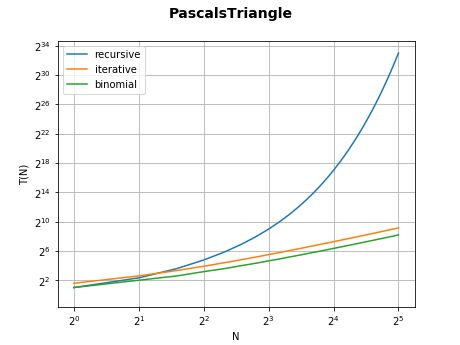
\includegraphics[width=\textwidth]{./IMG/PascalsTriangle.png}
    \caption[recur iter fast]{Die Aufwende der Implementationen des rekursiven, iterativen und die über den Binomialkooeffizienten Algorithmen sind gegen die Dreieckstiefe N aufgetragen.}
\end{figure}
	
In Abbildung \ref{fig:iterfast} sind nur die iteration und der schnelle Algorithmus auf Basis des Binominal Koeffizienten. Beide Algorithmen haben die selbe Komplexität, jedoch hat die binominale Version allgemein einen kleineren Aufwand. Die Komplexität von $\mathcal{O}(N^2)$ kann man mit der Steigungsdreieckmethode im loglog-Diagramm nachzählen.
	
\begin{figure}[htp]
	\label{fig:iterfast}
  	\centering
    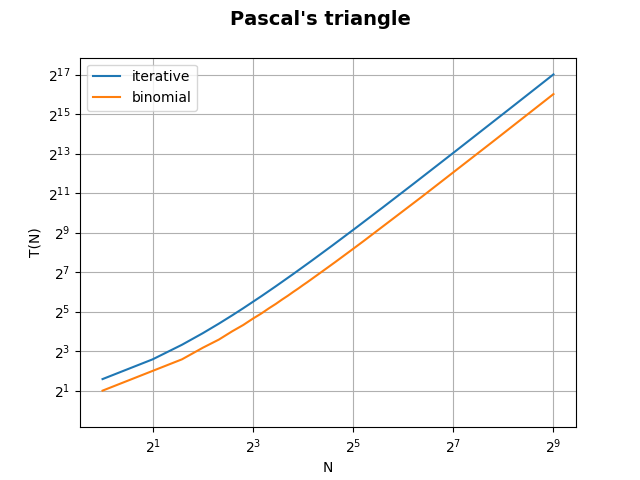
\includegraphics[width=\textwidth]{./IMG/iterfast.png}
    \caption[iter fast]{Die Aufwende des iterativen und die angeblich schnellere Implementation über den Binomialkooeffizienten sind gegen die Dreieckstiefe N aufgetragen.}
\end{figure}




\end{document}
% vim: set spell spelllang=de :EOF
